% SciTech 2027 final paper -- working draft.
% Scope note for the authors: the submitted extended abstract also promised ship-airwake results
% over multiple wind-over-deck conditions. Those are OUT of this paper (decision 2026-10-12); the
% paper covers the lid-driven cavity (Re 15k, 30k) and the Challenge 2.1 cavity PIV.
% Numbers in this draft come from results/*/saved_metrics, results/ldc_15k_dls_p99m10/
% reassembly_study_heldout.json and results/cavity_challenge_eval.json (scripts/challenge_eval.py).
% Red \todo{} marks results that are still running or not yet done.
\documentclass[conf]{new-aiaa}
\usepackage[utf8]{inputenc}

\usepackage{graphicx}
\usepackage{amsmath}
\usepackage{bm}
\usepackage{booktabs}
\usepackage{multirow}
\usepackage{xcolor}
\usepackage{siunitx}
\usepackage{longtable,tabularx}
\setlength\LTleft{0pt}

\graphicspath{{figs/}{../../figures/}{../lit_review/figs/}}
% keep floats near their text: looser placement limits, and no float crosses a section boundary
\usepackage[section]{placeins}
\renewcommand{\topfraction}{0.9}
\renewcommand{\bottomfraction}{0.8}
\renewcommand{\textfraction}{0.1}
\renewcommand{\floatpagefraction}{0.75}
\setcounter{totalnumber}{4}

\newcommand{\todo}[1]{\textcolor{red}{[TODO: #1]}}
\newcommand{\Rey}{\mathrm{Re}}
\newcommand{\dvec}{\mathbf{d}}
\newcommand{\dhat}{\hat{\mathbf{d}}}

\title{Localized Latent-Space Forecasting for Transformer-Based Turbulence Surrogates}

\author{Caleb A. Morton\footnote{Graduate Research Associate, Department of Mechanical \& Aerospace Engineering, morton.311@osu.edu, Student Member AIAA.} and Jack J. McNamara\footnote{Professor, Department of Mechanical \& Aerospace Engineering, mcnamara.190@osu.edu, Associate Fellow AIAA (Corresponding Author).}}
\affil{The Ohio State University, Columbus, Ohio, 43210}
\author{Rohit Deshmukh\footnote{Assistant Professor, Department of Mechanical \& Aerospace Engineering, rohit.deshmukh@ucf.edu.}}
\affil{University of Central Florida, Orlando, Florida, 32816}

\begin{document}

\maketitle

\begin{abstract}
Transformer surrogates for turbulent flows are commonly trained on a single global latent vector per time step, so the network must learn correlations across the whole domain at once. We instead use a data-enriched finite element basis, the Data-informed Local Subspace (DLS), as a tokenizer: each element of a coarse mesh becomes one token that carries its local enrichment coefficients, and a transformer attends across elements to forecast every element's next state. Treating the latent space as a finite element space has two consequences that we exploit. First, the element mass matrix gives the field energy of any latent error, and we use it in both the training loss and the evaluation. Second, independently predicted elements must be combined into one continuous field. A mass-weighted least-squares projection does this better than the nodal averaging used previously, and training through it makes the forecasts more consistent across seeds. For the lid-driven cavity at a Reynolds number of 15,000, with four times fewer latent coefficients than our prior work, the element-token model outperforms a global temporal transformer on the same latent space. Its mean 30-step relative field error over 50 held-out forecasts is 3.8\%, against 32.4\% for persistence, and its 500-step root-mean-square velocity field is within 1.4 percentage points of the compression floor, over three random seeds. At a Reynolds number of 30,000 the same recipe overfits a short training record. A longer record raises the 30-step skill over persistence from 0.02 to 0.33, but the long rollout loses a third of its energy, and a frequency-extrapolation baseline with no forecast skill reproduces the root-mean-square velocity field more closely. On the Challenge 2.1 cavity PIV, scored with the official metric on held-out sequences, a 1.9-million-parameter version of the model reaches a mean 30-step normalized mean-square error of 0.77 over three seeds, against 1.09 for the dynamic mode decomposition baseline and 1.0 for the mean flow, and stays below the mean-flow forecast at every lead time. Its forecasts lose amplitude as they lose predictability. We show that this is the error-optimal response of a deterministic model, that an energy penalty restores the amplitude but not the spectrum, and that long free rollouts settle onto a single Rossiter tone of the cavity that carries a fifth of the fluctuating energy.
\end{abstract}

\section*{Nomenclature}

{\renewcommand\arraystretch{1.0}
\noindent\begin{longtable*}{@{}l @{\quad=\quad} l@{}}
$\mathbf{B}$ & element basis matrix, local DLS shape functions sampled on the element's grid points \\
$\dvec$, $\dvec_e$ & global and element-local latent coefficient (DOF) vectors \\
$\dhat_e$ & element-local coefficients predicted by the network \\
$E$ & number of finite elements (tokens) \\
$\mathbf{G}_e$ & Boolean gather matrix, $\dvec_e = \mathbf{G}_e\dvec$ \\
$H$ & forecast horizon, steps \\
$\mathbf{M}_e$, $\mathbf{M}$ & element and assembled mass (Gram) matrices of the DLS basis \\
$m$ & number of local POD enrichment modes per node \\
$N_i$ & bilinear finite element shape function of node $i$ \\
$n_\mathrm{skip}$ & grid points between finite element nodes \\
$\Rey$ & Reynolds number \\
$S$ & forecast skill relative to persistence \\
$\mathbf{u}'$ & fluctuating velocity field \\
$\mathbf{W}$, $\mathbf{W}_e$ & diagonal grid-point weights of an element (zero outside the domain for cut elements) \\
$\varepsilon_k$ & relative field error after $k$ forecast steps \\
$\lambda$ & regularization of the assembly and loss metrics \\
$\tau$ & number of input snapshots (context length) \\
$\psi_k$ & $k$th local POD enrichment mode
\end{longtable*}}

%=====================================================================================
\section{Introduction}
\lettrine{D}{ata-driven} surrogate models are an attractive way to accelerate the analysis and prediction of turbulent flows. High-fidelity simulations and time-resolved measurements produce datasets that are expensive to generate, store, and analyze, and the cost of the underlying computation becomes prohibitive in many-query settings such as design studies, uncertainty quantification, and real-time or control-oriented applications \cite{benner2015survey}. A common strategy is to first compress each snapshot into a low-dimensional latent state and then learn the evolution of that state. Compression makes learning tractable: the number of trainable parameters, the amount of data required, and the cost of each forecast step all scale with the latent dimension rather than with the number of grid points \cite{brunton2020ml,vinuesa2022enhancing,brunton2024promising}.

Reduced-order models have traditionally emphasized the smallest latent state that represents the flow. Global modal decompositions such as proper orthogonal decomposition (POD) \cite{sirovich1987,berkooz1993,holmes2012turbulence,taira2017modal,taira2020modal} achieve this when a few energetic coherent structures dominate the flow. Their compactness degrades for high-Reynolds-number turbulence with a wide range of spatial scales, for convection-dominated flows \cite{mojgani2017lagrangian}, and when operating conditions change \cite{deshmukh2016sparse}. Correlations in turbulent flows decay with separation, so a global mode that represents a structure in one region spends degrees of freedom everywhere else. Localized representations avoid this. Earlier approaches treated difficult regions separately \cite{lucia2001thesis}, built local bases in state space \cite{amsallem2012local}, or decomposed the domain into subdomains with their own bases \cite{hoang2021ddlspg,diaz2024ddnm}. The Data-informed Local Subspace (DLS) method of Deshmukh et al.~\cite{deshmukh2020dls} combines the generalized finite element method (GFEM) \cite{melenk1996pum,babuska2004gfem} with local POD modes learned from snapshot data. The result is a compactly supported, $C^0$-continuous basis that reuses the same small set of local modes everywhere in the domain.

Neural-network autoencoders offer nonlinear compression \cite{gonzalez2018deep,lee2020cae,eivazi2022betavae}, and recurrent networks \cite{srinivasan2019,eivazi2021koopman,borrelli2022channels,vlachas2020backprop}, Koopman embeddings \cite{lusch2018koopman}, and transformers \cite{vaswani2017attention,wu2022transformer,solera2024betavae,geneva2022transformers,hemmasian2023transformers,sarma2024tbl} have been used to evolve the resulting latent states. These models typically forecast one global latent vector per time step, and autoregressive forecasting of turbulence remains difficult because errors compound over the rollout and the truncated latent state may not be closed \cite{linot2023stabilized,kohl2023acdm,lippe2023pderefiner}. Finite element spaces have also entered learned surrogates. Operator networks predict finite element coefficients for parametric PDEs \cite{lee2025feonet,chawla2026dgfeonet,franco2023minn}, mesh-based models roll unsteady flows out in time \cite{gao2024hypergraph,lu2026graphrom}, and networks have been paired with local reduced bases \cite{wang2019gmsfem,pan2024ddpdcnn}. We are not aware of a learned forecasting model, other than our earlier work \cite{morton2026scitech}, whose latent state is the coefficient vector of a data-enriched finite element basis.

Our previous work \cite{morton2026scitech} trained transformers on DLS and POD latent spaces of a lid-driven cavity at Reynolds numbers of 15,000 and 30,000. DLS latents preserved long-time turbulence statistics better than POD latents of comparable size, but a simple frequency-domain extrapolation of the latent coefficients matched the transformer. That study localized the representation but not the forecast: the transformer received the entire latent vector, 10,648 coefficients, and predicted all of it at once. This paper poses the forecast locally. Each finite element becomes one token, in the same way that vision transformers tokenize image patches \cite{dosovitskiy2021vit} and that recent neural surrogates tokenize spatial locations or latent anchors \cite{serrano2024aroma,alkin2024upt}. A transformer attends across the element tokens and predicts each element's next state. No governing equations enter the forecast. The finite element structure is retained because it supplies two things a generic tokenizer does not: an exact energy metric on the latent space, and an assembly operator that turns independent element predictions into one conforming field. We also move to stronger compression, with 2,662 coefficients for the lid-driven cavity, and report the compression floor alongside every result so that forecasting error and compression error can be separated.

Neither ingredient is new in itself. The mass matrix gives the $L^2$ norm of a finite element function, and it has been used in the training losses of mesh-informed networks \cite{franco2023minn} and of a domain-decomposed reduced model for steady elliptic problems \cite{dimola2026ddrom}; the latitude-weighted loss of GraphCast \cite{lam2023graphcast} is its diagonal analogue. A least-squares projection of element-wise data onto a continuous field is the classical alternative to nodal averaging in finite element stress recovery \cite{hinton1974smoothing}. What differs here is where they act. The DLS latent state is compressed, enriched, and far from orthogonal, so its mass matrix is severely ill-conditioned and must be regularized (Sec.~\ref{sec:gram}). The projection is applied to learned element predictions inside an autoregressive rollout, including during training, which to our knowledge has not been done before. Following recommended evaluation practice \cite{mcgreivy2024weak}, all results are on a contiguous held-out time window, are compared against persistence and the compression floor, and are repeated over three random seeds for the headline recipes. The short-horizon protocol mirrors the forecasting track of the community challenge of Schmidt et al.~\cite{schmidt2026challenge}.

The contributions of this paper are:
\begin{enumerate}
  \item an element-token formulation of latent forecasting on a data-enriched finite element basis, with attention over space and one token per element;
  \item the use of the regularized DLS mass (Gram) matrix as the field-energy metric for the training loss and the evaluation of a forecasting model in a compressed, non-orthogonal latent space; and
  \item a mass-weighted least-squares projection that assembles independently predicted elements, with nodal averaging as a limiting case, applied inside the multi-step training rollout.
\end{enumerate}
The model is evaluated on the lid-driven cavity at two Reynolds numbers and on the Challenge 2.1 cavity PIV, where we also show why deterministic forecasts lose amplitude as predictability is lost.

%=====================================================================================
\section{Data-Informed Local Subspace Latent Space}
\label{sec:dls}

\subsection{Construction}
DLS \cite{deshmukh2020dls} embeds data-driven local modes in a GFEM approximation \cite{melenk1996pum,babuska2004gfem}. A coarse mesh of bilinear finite elements, with nodes every $n_\mathrm{skip}$ grid points, is laid over the data grid. Its shape functions $N_i$ form a partition of unity, and each $N_i$ is supported on the patch $\omega_i$ of the elements that share node $i$. Patches of $(2n_\mathrm{skip}+1)^2$ grid points are sampled at random locations from a single training snapshot (the first of the record), their means are removed, and POD of the sampled patches gives $m$ local modes $\psi_k$. Because the local modes need only one snapshot, the basis never sees the held-out data. The same modes are used at every node, centered on the node so that their footprint covers $\omega_i$. The fluctuating velocity is then approximated as
\begin{equation}
  \mathbf{u}'(\mathbf{x},t)\approx\sum_{i}N_i(\mathbf{x})\Bigl[a_i(t)+\sum_{k=1}^{m}b_{ik}(t)\,\psi_k(\mathbf{x}-\mathbf{x}_i)\Bigr],
  \label{eq:gfem}
\end{equation}
separately for each velocity component. Each enrichment $N_i\psi_k$ vanishes on the boundary of $\omega_i$, so the representation is $C^0$-continuous. Every node therefore carries $m+1$ coefficients per component. The coefficients of a snapshot are obtained by $L^2$ projection onto the enriched space, i.e., by assembling and solving the global system $\mathbf{M}\dvec=\mathbf{P}$, where $\mathbf{P}$ is the projection of the snapshot onto the basis \cite{deshmukh2020dls}. Figure~\ref{fig:dls} illustrates the construction in one dimension.

\begin{figure}[!tbp]
  \centering
  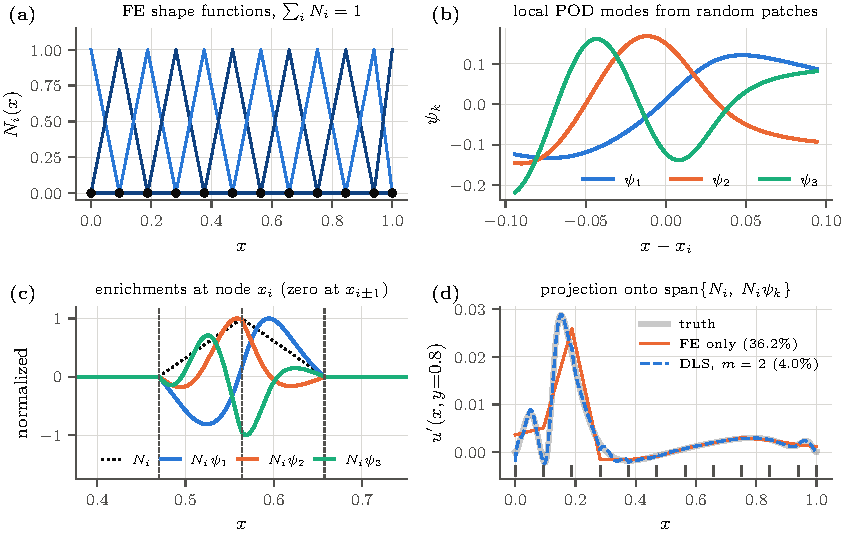
\includegraphics[width=0.85\textwidth]{dls_schematic.pdf}
  \caption{DLS construction in one dimension. (a) Finite element shape functions forming a partition of unity. (b) Local POD modes obtained from randomly sampled patches. (c) Enrichments $N_i\psi_k$ at one node; they vanish at the neighboring nodes. (d) Projection of a cavity velocity profile onto the shape functions alone and onto the enriched space.}
  \label{fig:dls}
\end{figure}

\subsection{Element-local structure and the field-energy metric}
\label{sec:gram}
The reconstruction is linear and block-diagonal by element. Let $\dvec_e=\mathbf{G}_e\dvec$ gather the $n_e=4(m+1)$ coefficients per component of the four nodes of element $e$. The field over the element is then $\mathbf{u}_e=\mathbf{B}\dvec_e$. Here $\mathbf{B}$ holds the products $N_i\psi_k$ sampled on the element's grid points, and it is the same for every element of a uniform mesh. Grid points on shared element edges and corners are weighted by a diagonal matrix $\mathbf{W}$ that splits them among the elements that contain them. The field energy of any coefficient vector is then exactly
\begin{equation}
  \|\mathbf{u}\|^2=\sum_{e=1}^{E}\dvec_e^{\top}\mathbf{M}_e\dvec_e=\dvec^{\top}\mathbf{M}\dvec,\qquad
  \mathbf{M}_e=\mathbf{B}^{\top}\mathbf{W}\mathbf{B},\qquad
  \mathbf{M}=\sum_{e}\mathbf{G}_e^{\top}\mathbf{M}_e\mathbf{G}_e .
  \label{eq:gram}
\end{equation}
The coefficients therefore live in the $\mathbf{M}$ metric, not the Euclidean one. The distinction is large in practice. For the production basis used below, $\mathbf{B}$ has a condition number of $3.2\times10^{5}$ and the assembled $\mathbf{M}$ has a condition number of $2.5\times10^{10}$. Many coefficient directions carry almost no field energy, and a mean-squared error on raw coefficients is dominated by them. For real model errors, the gradient of a mean-squared error on the standardized coefficients lies $83$--$86^\circ$ from the gradient of the field-energy error, on both bases used below. It still descends, because $\mathbf{M}$ is positive semidefinite, but very inefficiently.

We use Eq.~\eqref{eq:gram} in three places. The training loss scores the element errors in a regularized element metric,
\begin{equation}
  \mathcal{L}=\frac{1}{H_\mathrm{tr}}\sum_{k=1}^{H_\mathrm{tr}}\sum_{e=1}^{E}\bigl\|\mathbf{R}_\lambda\bigl(\dhat_e^{(k)}-\dvec_e^{(k)}\bigr)\bigr\|^2,\qquad
  \mathbf{R}_\lambda=\Bigl(\mathbf{M}_e+\lambda\,\tfrac{\operatorname{tr}\mathbf{M}_e}{n_e}\mathbf{I}\Bigr)^{1/2},
  \label{eq:loss}
\end{equation}
summed over both velocity components. With $\lambda=0$ this is exactly the field energy of the error. The ridge is needed because the near-null directions of $\mathbf{M}_e$ are invisible in the field but are fed back to the network as inputs. With nothing constraining them, they drift during autoregressive rollouts. We use $\lambda=10^{-2}$ throughout. The value is a trade-off between the short horizon and the long one. Over three seeds on a full-coverage variant of the $\Rey=15{,}000$ basis (Sec.~\ref{sec:fullcover}), $\lambda=10^{-4}$ lowered the 30-step mean error from $0.027$ to $0.017$ but raised the 500-step RMS error from 6.3\% to 8.4\% and the TKE error from 1.6\% to 5.0\%. Below $10^{-4}$ the rollout gains energy, to 3.4 and 21 times the truth at $10^{-5}$ and $10^{-6}$ (one seed each).
The ridge is not a small correction. The true coefficients are large along the ill-conditioned directions, because a modest field component along such a direction needs a large coefficient. At $\lambda=10^{-2}$ the ridge therefore carries 99.8\% of the metric norm of the true $\Rey=15{,}000$ coefficients, and 77\% for the better-conditioned Challenge 2.1 basis (Sec.~\ref{sec:challenge}). The loss is the field-energy error plus a penalty on the coefficients. Terms that should act on the visible field alone, such as the energy term of Sec.~\ref{sec:tradeoff}, are therefore computed with $\lambda=0$. The unregularized metric scores forecast errors in Sec.~\ref{sec:eval}, and the regularized one, with the same $\lambda$, defines the assembly in Sec.~\ref{sec:assembly}. Evaluating Eq.~\eqref{eq:gram} costs one $n_e\times n_e$ product per element, so no field needs to be decoded.

\subsection{Covering the whole grid}
\label{sec:fullcover}
A uniform mesh with nodes every $n_\mathrm{skip}$ grid points covers an $n_x\times n_y$ grid only when $n_x-1$ and $n_y-1$ are multiples of $n_\mathrm{skip}$. Otherwise the trailing rows and columns lie outside every element and are dropped. For the lid-driven cavity mesh this is a 21-point strip along the right wall and along the lid, and the lid-driven cavity results in this paper are computed on the $491\times491$ region that the mesh covers. The Challenge 2.1 metric is scored on every grid point, so there we extend the mesh by one row or column of nodes past the edge and give the grid points outside the domain zero weight in each element's mass matrix, $\mathbf{M}_e=\mathbf{B}^{\top}\mathbf{W}_e\mathbf{B}$. The extended mesh has 234 elements and 3,240 coefficients instead of 200 and 2,808. It represents all $154\times51$ points with the same compression error as the truncated mesh has over the region it covers (normalized mean-square error 0.036). In the basis used below, the compression solve also fits the points outside the domain, with weight 0.1, to an odd reflection of the field about the boundary. Over three seeds this changed no result measurably.

\subsection{Latent spaces considered}
Table~\ref{tab:latent} lists the lid-driven cavity bases. The present basis uses $99\times99$ patches ($n_\mathrm{skip}=49$), which on the $512\times512$ grid gives a $10\times10$ element mesh covering $491\times491$ grid points, and $m=10$ local modes, for 2,662 coefficients. The basis of Ref.~\cite{morton2026scitech} used $49\times49$ patches and ten modes, for 10,648 coefficients. The compression floor is the RMS-velocity error of the DLS reconstruction of the true snapshots over the evaluation window. It bounds what any forecast in that latent space can achieve.

\begin{table}[!tbp]
  \centering
  \small
  \caption{DLS latent spaces for the lid-driven cavity at $\Rey=15{,}000$.}
  \label{tab:latent}
  \begin{tabular}{lccccccc}
    \toprule
    Basis & Patch & $m$ & Nodes & Elements & Coefficients & Points per coefficient\textsuperscript{a} & RMS floor, \% \\
    \midrule
    Ref.~\cite{morton2026scitech} & $49^2$ & 10 & $22\times22$ & 441 & 10,648 & 48 & 0.6 \\
    p99m10 (this work) & $99^2$ & 10 & $11\times11$ & 100 & 2,662 & 181 & 4.28 \\
    \bottomrule
  \end{tabular}

  \smallskip
  {\footnotesize \textsuperscript{a}Grid points covered by the mesh per coefficient of one velocity component.}
\end{table}

%=====================================================================================
\section{Forecasting on Element Tokens}
\label{sec:model}

\subsection{Spatial transformer}
Each of the $E=100$ elements becomes one token. The token holds the element's coefficients for both velocity components over the last $\tau=4$ snapshots, $2n_e\tau=352$ values for p99m10. Each coefficient is standardized over the training set. A linear layer projects the token to the model width $d=256$. A Fourier-feature embedding of the element centroid \cite{tancik2020fourier}, with six octave-spaced frequencies per coordinate, is added to it. Four pre-normalized \cite{xiong2020layer} transformer encoder layers with four heads and SwiGLU feed-forward blocks of width 768 \cite{shazeer2020glu} then attend across all elements. A final normalization and linear head map each token to its element's next-step coefficients. The head predicts a residual: its output is added to the most recent input frame, and its weights are initialized to zero, so the untrained model is persistence. The model has 7.48 million parameters. For the Challenge 2.1 cavity we also use a narrower version (width 128, feed-forward width 384; 1.88 million parameters), which forecasts as well as the full one (Sec.~\ref{sec:res_challenge}).

Time enters only through the stacked frames in each token, and attention runs over space. Because no attention runs across time, the model needs no temporal positional encoding such as rotary embeddings \cite{su2024roformer}. Element position is supplied by the coordinate embedding. Every element attends to every other, so each local prediction can draw on the state of the whole cavity. What is local is the representation: each output is the update of one element's coefficients, and the same weights are shared by all elements. Figure~\ref{fig:arch} shows one step of the forecast.

\begin{figure}[!tbp]
  \centering
  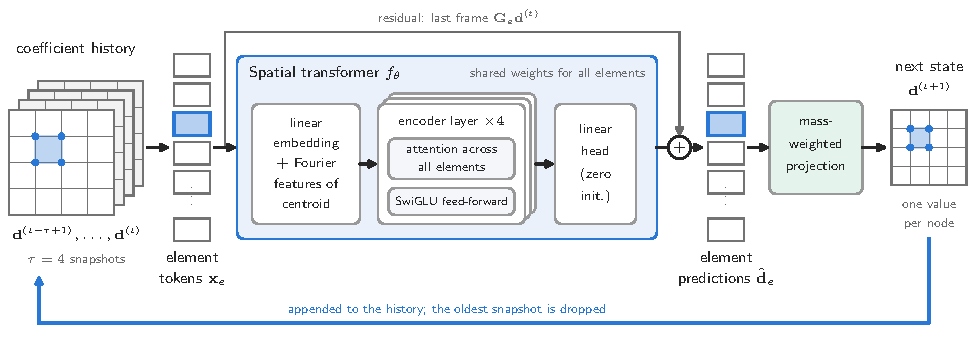
\includegraphics[width=\textwidth]{model_schematic.pdf}
  \caption{One step of the element-token forecast. The last $\tau$ coefficient snapshots are gathered into one token per element. The spatial transformer attends across all elements and predicts each element's next coefficients as a residual on its last frame. The mass-weighted projection of Sec.~\ref{sec:assembly} combines the element predictions into one coefficient vector, which is appended to the history.}
  \label{fig:arch}
\end{figure}

\subsection{Assembling element predictions}
\label{sec:assembly}
Each node is shared by up to four elements, and each of those elements predicts the node's coefficients independently. The predictions are not identical, so they must be combined into one global coefficient vector before the next step. If they are not, the copies drift apart. Figure~\ref{fig:reassembly}a shows the mismatch at shared nodes in a rollout without assembly: it grows to 44\% of the predicted frame's energy by step 500. The original formulation averaged each node's copies. This is least squares in the raw coefficient metric, which, as shown in Sec.~\ref{sec:gram}, is not the metric of the field.

Finite element assembly instead projects the discontinuous element-wise field onto the conforming space in the field metric. We use a regularized version,
\begin{equation}
  \dvec^{\star}=\arg\min_{\dvec}\sum_{e}\bigl(\mathbf{G}_e\dvec-\dhat_e\bigr)^{\top}\mathbf{M}_{e,\lambda}\bigl(\mathbf{G}_e\dvec-\dhat_e\bigr)
  \;\Longrightarrow\;
  \Bigl(\sum_{e}\mathbf{G}_e^{\top}\mathbf{M}_{e,\lambda}\mathbf{G}_e\Bigr)\dvec^{\star}=\sum_{e}\mathbf{G}_e^{\top}\mathbf{M}_{e,\lambda}\dhat_e,
  \label{eq:assembly}
\end{equation}
with $\mathbf{M}_{e,\lambda}=\mathbf{M}_e+\lambda\,(\operatorname{tr}\mathbf{M}_e/n_e)\,\mathbf{I}$. We call Eq.~\eqref{eq:assembly} the mass-weighted projection. It projects the predicted field onto the DLS space; unlike the Galerkin projection of POD-based reduced-order models, it involves no governing equations. The family contains both existing choices. As $\lambda\rightarrow\infty$ the metric becomes the identity, and Eq.~\eqref{eq:assembly} reduces to the nodal average. With $\lambda=0$ it is the pure $L^2$ projection, which decodes each element and re-encodes the field. The pure $L^2$ projection is unstable in a rollout. The near-null directions of $\mathbf{M}$ are almost free under the field metric, so the projection injects large coefficients along them; these are invisible in the field but feed back through the network's inputs. Intermediate values of $\lambda$ remove inter-element disagreement in the field metric while keeping a floor under every direction. We use $\lambda=10^{-2}$, the same value as in the loss. On a full-coverage mesh (Sec.~\ref{sec:fullcover}) each cut element uses its own $\mathbf{M}_e$, and every ridge is scaled by the trace of a full element, so the weakly observed coefficients of cut elements are held as firmly as interior ones. The left-hand matrix of Eq.~\eqref{eq:assembly} is fixed, so its inverse is computed once (1,331 unknowns per velocity component for p99m10). Each step then costs one matrix--vector product per component, a negligible fraction of a transformer forward pass, and the whole operation is linear and therefore differentiable.

The operation itself is classical. A global least-squares projection of discontinuous element-wise data onto a continuous nodal field is the standard alternative to nodal averaging for recovering smooth stresses from finite element solutions \cite{oden1971consistent,hinton1974smoothing,zienkiewicz1992spr}, and the ridge is a Tikhonov regularization \cite{tikhonov1977illposed,hoerl1970ridge}. Learned mesh-based and domain-decomposed models have so far reconciled nodes duplicated on element boundaries by averaging \cite{barwey2024consistent,sankaran2025elementlocal,pan2024ddpdcnn}. To our knowledge, a mass-weighted projection has not previously been used to combine learned element predictions, nor has a surrogate been trained through one.

The assembly can be applied only at inference, or inside the training rollout as well. In the second case the loss scores the assembled state, and the network is trained on the consistent states it receives at inference. Both variants are evaluated in Sec.~\ref{sec:res_assembly}.

\subsection{Training}
The model is trained by free-running multi-step rollouts. Each training sample is a window of $\tau+H_\mathrm{tr}$ consecutive snapshots with $H_\mathrm{tr}=16$. The model is seeded with the first $\tau$ true frames and then fed its own (assembled) predictions. The loss of Eq.~\eqref{eq:loss} is accumulated at every step. Gradients propagate through the rollout by truncated backpropagation through time \cite{werbos1990} in chunks of eight steps, with gradient checkpointing \cite{chen2016checkpoint} to keep memory constant in the rollout depth. The backpropagation depth grows from one step to eight over the first 20 epochs, because a freshly initialized model rolled out many steps produces non-finite gradients. Training on multi-step rollouts, rather than single steps, is known to improve the stability of autoregressive neural surrogates \cite{brandstetter2022mpnn,vlachas2020backprop}. It is essential here. A model trained on teacher-forced single steps had an accurate first step ($\varepsilon_1=0.008$, against 0.006 for the multi-step model), but its 496-step rollout grew to 570 times the true fluctuating energy. Additional penalties on the trajectory's energy, variance, and time derivative degraded the 30-step error (0.130 against 0.072) and are not used.

We use Adam \cite{kingma2015adam} with a learning rate of $10^{-3}$, halved after five epochs without improvement on the test split, batches of 64 windows, gradient clipping at a norm of one, and mixed precision. Training stops when the test loss has not improved by 1\% for ten epochs. On the $\Rey=15{,}000$ data this takes 73--102 epochs and under 70 minutes on a single NVIDIA RTX 3090 Ti.

%=====================================================================================
\section{Evaluation Protocol}
\label{sec:eval}

\subsection{Held-out split}
Each record is split into three contiguous blocks in time: training $[0,a)$, test $[a,b)$, and evaluation $[b,T)$. The evaluation block holds the last 20\% of the record, the test block the preceding 10\% of the remainder, and the training block everything before it. Every training window lies entirely in the training block, and every test window in the test block. The test block is used only for early stopping and learning-rate control, and the evaluation block is never seen during training or model selection. For the $\Rey=15{,}000$ cavity, training windows cover snapshots 0--1799, test windows 1800--1998, and evaluation 1999--2498. The architecture comparison of Sec.~\ref{sec:res_arch} used an earlier split in which the early-stopping windows overlapped the training data. The evaluation block was held out in both, and re-running the headline recipes on the corrected split changed their skill by less than 0.01.

\subsection{Short-horizon forecasts}
A single long rollout starts from one initial condition, so any spread it shows is over time steps, not over forecasts. We therefore launch $N_s=50$ forecasts of $H=30$ steps from starting points spread evenly across the evaluation block. Each forecast is seeded with $\tau$ true frames. The error after $k$ steps is the relative field error
\begin{equation}
  \varepsilon_k=\frac{\|\dhat^{(k)}-\dvec^{(k)}\|_{\mathbf{M}}}{\|\dvec^{(k)}\|_{\mathbf{M}}},\qquad \|\dvec\|_{\mathbf{M}}^2=\dvec^{\top}\mathbf{M}\dvec ,
  \label{eq:err}
\end{equation}
where $\dvec^{(k)}$ is the DLS projection of the true fluctuating field. Through Eq.~\eqref{eq:gram} this is the exact field-space $L^2$ error. We verified it against full $491\times491$ reconstructions, which agreed to a median of 0.36\%. Because the reference is the projected truth, $\varepsilon_k$ measures forecasting error alone; compression error is reported separately as the floor in Table~\ref{tab:latent}. We report the mean of $\varepsilon_k$ over forecasts and steps, $\bar\varepsilon$, the per-step mean and spread, and the standard deviation across forecasts of each forecast's window-mean error, $\sigma_\mathrm{start}$. The challenge's normalized mean-square error \cite{schmidt2026challenge} is $\varepsilon_k^2$ evaluated on the challenge's own field.

Persistence, which holds the last seed frame, is the reference. On this cavity the field changes by about 2.1\% per snapshot, so persistence scores $\varepsilon_1=0.021$ and $\varepsilon_{30}=0.62$, and any forecast with a one-step error near 0.1 is worse than doing nothing. The skill is $S=1-\bar\varepsilon/\bar\varepsilon_\mathrm{persist}$: $S=0$ is persistence and $S=1$ is a perfect forecast.

\subsection{Long-horizon statistics}
Beyond the 30-step window, each model is rolled out freely for 496 steps from the start of the evaluation block (about five convective time units). The predicted coefficients are decoded, and we compare the following against the original data: the RMS velocity field, the turbulent kinetic energy (TKE) time history, the ratio of predicted to true fluctuating energy, and velocity spectra and probability densities at probes. RMS and TKE errors are relative $L^2$ errors against the DNS. They therefore include the compression floor.

An RMS or TKE error mixes amplitude, location, and scale, and it gives no indication of how close two records of the same flow can be. For the Challenge 2.1 cavity we therefore also compare the free rollout and the true flow over the same block using five statistics, each chosen to isolate one property of the fluctuating velocity:
\begin{enumerate}
  \item the energy ratio, the mean predicted-to-true fluctuating energy (amplitude);
  \item the relative $L^2$ error of the RMS-velocity map (where the fluctuations are);
  \item the log-spectral distance, in decibels, between the streamwise wavenumber spectra, each normalized by its total and summed in octave bands (how the energy is distributed across spatial scales, with amplitude removed);
  \item the same distance for the frequency spectra, computed by Welch's method at every fourth grid point, which contain the Rossiter tones (the distribution across time scales);
  \item the Wasserstein-1 distance between one-point velocity distributions after each record is standardized by its own local standard deviation, averaged over grid points (the shape of the distribution, including skewness and tails, with amplitude removed).
\end{enumerate}
None of these depends on timing, so a forecast is not penalized for losing phase with the truth. Each distance is divided by a sampling floor: the mean distance between the held-out truth and eight equally long segments of the training record. A ratio of 1 means that the forecast is as close to the truth as another stretch of the true flow. The floors themselves vary across segments by 9\% (distribution shape) to 51\% (spatial spectrum) of their means, so ratios below about 2 do not separate models. The DLS projection of the truth gives a second reference, the closest that any forecast in that basis can come. The spectral distances include every band. In this PIV record the content at wavelengths below about ten grid points, 5\% of the fluctuating energy, is uncorrelated from one frame to the next (lag-one coherence below 0.05, against 0.9 at the largest scales), so no forecast can predict it. Where a difference lies mainly in these bands, we say so.

\subsection{Seeds}
Headline recipes are trained with three random seeds, which change the weight initialization, the dropout masks, and the order of the training windows. We report the mean $\pm$ one standard deviation across seeds. Run-to-run differences from nondeterministic GPU kernels are about $10^{-7}$ in $\bar\varepsilon$ and are negligible.

%=====================================================================================
\section{Flow Configurations}
\label{sec:flows}
Figure~\ref{fig:datasets} shows one snapshot of each flow with its DLS element mesh.


\subsection{Lid-driven cavity}
The lid-driven cavity data are from direct numerical simulation of the nondimensional incompressible Navier--Stokes equations in a unit square, discretized on a $512\times512$ uniform grid, at $\Rey=15{,}000$ and $30{,}000$ \cite{deshmukh2016sparse,morton2026scitech}, with the sharp-interface immersed boundary solver of Mittal et al.~\cite{mittal2008versatile}. Both records are sampled at 100 snapshots per nondimensional time unit. The $\Rey=15{,}000$ record has 2,499 snapshots. The $\Rey=30{,}000$ record has 60,000 snapshots. We use its first 4,500 and first 10,000 snapshots and compress only the snapshots that are used, so the 10,000-snapshot study also changes the length of the evaluation block.

\subsection{Challenge 2.1 cavity PIV}
\label{sec:challenge}
The second dataset is the time-resolved PIV of a Mach 0.6 open-cavity flow by Zhang et al.~\cite{zhang2020samm}, used in Challenge 2.1 of the community challenge \cite{schmidt2026challenge}. The cavity has a length-to-depth ratio of 6, and the Reynolds number based on its depth is about $3.3\times10^5$. The field of view is resolved by $154\times51$ points, and the snapshots are sampled at 16~kHz. The flow combines broadband turbulence, Rossiter tones, and measurement noise. Of the 16,000 snapshots, 12,800 are released for training. The remaining 3,200 form 32 test sequences of 100 snapshots; the first 70 snapshots of each are given, and the last 30 must be forecast. The official metric is the per-step normalized mean-square error (NMSE) of the mean-removed field, $\mathbb{E}\|\hat{\mathbf{q}}_k-\mathbf{q}_k\|^2/\mathbb{E}\|\mathbf{q}_k\|^2$, reported as the mean and standard deviation across sequences. The challenge baselines are dynamic mode decomposition (DMD) \cite{schmid2010dmd} with 25 modes fit to each sequence's 70 inputs, and an LSTM on 25 global POD coefficients.

We split the 12,800 training snapshots as in Sec.~\ref{sec:eval}, with the last 10\% held out: training windows lie in snapshots 0--10,367, test windows in 10,368--11,519, and evaluation in 11,520--12,799. The basis uses $13\times13$ patches ($n_\mathrm{skip}=6$) and five local modes. With the full-coverage mesh of Sec.~\ref{sec:fullcover} it has $27\times10$ nodes, 234 elements, and 3,240 coefficients, and its compression floor over the held-out block is an NMSE of 0.036. With the original mesh and the uncovered strip set to the mean flow, the floor is 0.042.

\begin{figure}[!tbp]
  \centering
  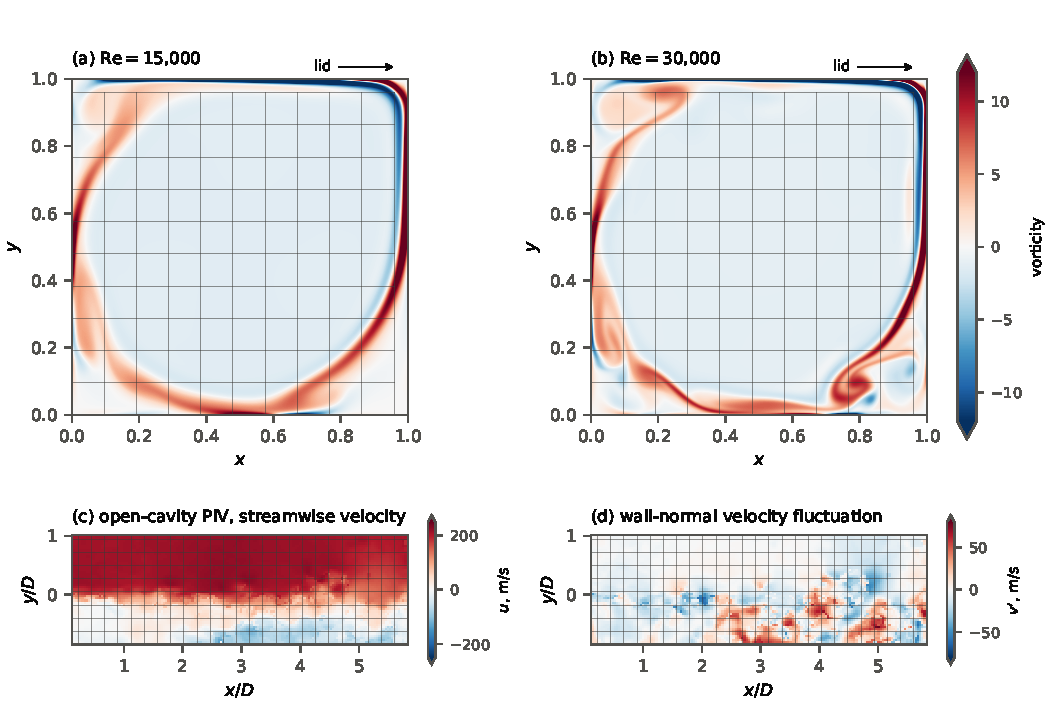
\includegraphics[width=\textwidth]{datasets.pdf}
  \caption{The flows studied, each with its DLS element mesh (thin lines; one element is one token). (a, b) Instantaneous vorticity of the lid-driven cavity at $\Rey=15{,}000$ and $30{,}000$; the mesh leaves a 21-point strip along the right wall and the lid uncovered. (c, d) One PIV snapshot of the Challenge 2.1 open cavity: streamwise velocity and wall-normal velocity fluctuation. The flow is from left to right and the cavity lies below $y/D=0$.}
  \label{fig:datasets}
\end{figure}

%=====================================================================================
\section{Results}
\label{sec:results}

\subsection{Global versus element-token forecasting}
\label{sec:res_arch}
Table~\ref{tab:arch} compares three architectures on the same p99m10 latent space, all trained with the field-energy loss and 16-step rollouts. The global temporal transformer, like Ref.~\cite{morton2026scitech}, treats the whole 2,662-coefficient vector as one token per time step and attends over 16 past steps. The global--local encoder--decoder encodes the element tokens of the most recent frame into a shared context and attends over time within each element. The spatial transformer of Sec.~\ref{sec:model} attends over elements only.

The element-token models forecast best over 30 steps. The spatial transformer improves on the global model in every metric, with a 30-step error of 0.072 against 0.125 and an RMS error of 6.9\% against 9.3\%, while using a larger but still modest network. The encoder--decoder has good short-horizon skill, but its long rollout gains energy (TKE error 28\%), so we do not pursue it further. The global model starts with a first-step error of 0.062, three times that of persistence, and its error then stays nearly flat near 0.055 for several steps; it beats persistence only from the third step. Both element-token models beat persistence from the first step.

The last row of Table~\ref{tab:arch} is the frequency-domain extrapolation that matched the transformer in Ref.~\cite{morton2026scitech}, applied to the same latent coefficients. It extends the Fourier series of each coefficient beyond the training block and takes no account of the current state, so it has no forecast skill: its error is 1.91 at every lead, six times that of persistence. Its long-run statistics are also worse than those of every transformer that remains stable, with an RMS error of 9.0\% and a TKE error of 14.8\%.

\begin{table}[!tbp]
  \centering
  \small
  \caption{Architecture comparison, $\Rey=15{,}000$, p99m10, single seed, nodal-average assembly. Persistence: $\bar\varepsilon=0.324$, $\varepsilon_{1}=0.021$, $\varepsilon_{30}=0.621$.}
  \label{tab:arch}
  \begin{tabular}{lccccccc}
    \toprule
    Model & Parameters & Attention over & $S$ & $\varepsilon_{1}$ & $\varepsilon_{30}$ & RMS error, \% & TKE error, \% \\
    \midrule
    Global temporal transformer & 2.53 M & time (16 steps) & 0.740 & 0.062 & 0.125 & 9.31 & 15.3 \\
    Global--local enc.--dec.\textsuperscript{a} & 8.23 M & elements, then time & 0.822 & 0.009 & 0.101 & 36.9 & 28.2 \\
    Spatial transformer & 7.48 M & elements & 0.854 & 0.006 & 0.072 & 6.94 & 1.85 \\
    \midrule
    Frequency extrapolation\textsuperscript{b} & -- & -- & $-4.88$ & 1.91 & 1.91 & 9.04 & 14.8 \\
    \bottomrule
  \end{tabular}

  \smallskip
  {\footnotesize \textsuperscript{a}Trained with additional penalties on the trajectory's energy, variance, and time derivative. \textsuperscript{b}Ref.~\cite{morton2026scitech}: Fourier series of each latent coefficient over the training block with every frequency kept, which repeats the training record; it uses no seed frames.}
\end{table}

\subsection{Assembly of element predictions}
\label{sec:res_assembly}
Table~\ref{tab:assembly} and Fig.~\ref{fig:reassembly} compare four ways of combining the element predictions, each over three seeds on the held-out split. In the first three rows the same trained weights are used, and only the inference-time assembly changes.

Without assembly, the 30-step skill is unchanged ($S=0.860$), but the copies of shared nodes drift apart. Their disagreement grows from $3\times10^{-5}$ to 44\% of the frame energy over 500 steps (Fig.~\ref{fig:reassembly}a), and the RMS error triples to 18.2\%. Short-horizon skill is therefore a poor guide to whether a model is fit for long forecasts. Nodal averaging holds the disagreement near $5\times10^{-5}$ and reduces the RMS error to 6.25\%.

The mass-weighted projection, applied to the same weights, improves every metric. The skill rises from 0.861 to 0.879, the 30-step error falls from 0.068 to 0.059, and the RMS error falls from 6.25\% to 5.74\%. The improvement holds in every seed. Training through the projection adds a smaller further gain, concentrated in the 30-step error ($0.053\pm0.001$) and in the consistency across seeds: the seed spread of the skill halves, and that of the 30-step error falls by a factor of three. The RMS error, 5.64\%, is 1.4 percentage points above the 4.28\% compression floor, against 2.0 points for nodal averaging.

Nodal averaging and the model trained through the projection both stay well below persistence throughout the 30-step window. Their errors are 3.4--3.7 times smaller at the first step and 9--12 times smaller at step 30, where they reach 0.068 and 0.053 against 0.62 for persistence. The model trained through the projection has a forecast-to-forecast spread of $\sigma_\mathrm{start}=0.0035$. It is slightly less accurate than nodal averaging at the first step (0.0062 against 0.0057) and more accurate from step four on. This is consistent with a projection that removes some of the network's one-step detail but keeps errors from compounding.

A model trained through the projection learns to rely on it. Thirty steps into a held-out rollout, its raw element outputs disagree along shared edges by 125\% of the field's RMS value and are 28\% from the truth; after the solve the edges agree to round-off and the error is 4.3\%. Because the loss only ever sees the projected state, the network's raw output is an intermediate rather than a forecast. A model trained on raw outputs produces nearly consistent elements (edge jumps of 1.2\%), and the projection barely changes its error at a single step (4.7\% before and after). For that model, the projection's benefit is that it stops the slow drift of Fig.~\ref{fig:reassembly}a.

Figure~\ref{fig:ldc_stats} shows the long-horizon behavior for seed 1. The RMS-velocity map of the forecast is indistinguishable by eye from those of the DNS and of its DLS projection. Over almost all of the domain the difference is more than an order of magnitude below the peak value, and it is largest near the walls (Fig.~\ref{fig:ldc_stats}d). Over the 496-step rollout both forecasts follow the slow variation of the fluctuating kinetic energy to within about 6\% (Fig.~\ref{fig:ldc_stats}e), and the model trained through the projection keeps the energy within 1\% of the truth on average ($1.007\pm0.008$ over seeds). Reference~\cite{morton2026scitech} reported RMS errors of $\mathcal{O}(1\%)$ at this Reynolds number with a basis whose own floor was 0.6\%. The present model works with four times fewer coefficients and a seven-times-higher floor, and it adds 1.4 percentage points to that floor.

The improvement is not uniform across statistics. The TKE error of the model trained through the projection is $2.11\pm0.46$\%, against $1.78\pm0.38$\% for nodal averaging; the ranges overlap. Its mean energy ratio is $1.007\pm0.008$, against $0.994\pm0.002$.

\begin{table}[!tbp]
  \centering
  \small
  \caption{Assembly study, $\Rey=15{,}000$, p99m10, held-out split, mean $\pm$ standard deviation over three seeds. Compression floor for the RMS error: 4.28\%. Persistence: $\bar\varepsilon=0.324$, $\varepsilon_{30}=0.621$.}
  \label{tab:assembly}
  \begin{tabular}{llcccc}
    \toprule
    Assembly at inference & Trained with & $S$ & $\bar\varepsilon$ & $\varepsilon_{30}$ & RMS error, \% \\
    \midrule
    None & raw outputs & $0.860\pm0.010$ & $0.045\pm0.003$ & $0.072\pm0.005$ & $18.2\pm0.7$ \\
    Nodal average & raw outputs & $0.861\pm0.010$ & $0.045\pm0.003$ & $0.068\pm0.004$ & $6.25\pm0.26$ \\
    Mass-weighted, $\lambda=10^{-2}$ & raw outputs & $0.879\pm0.010$ & $0.039\pm0.003$ & $0.059\pm0.004$ & $5.74\pm0.11$ \\
    Mass-weighted, $\lambda=10^{-2}$ & projection in the loop & $0.883\pm0.005$ & $0.038\pm0.002$ & $0.053\pm0.001$ & $5.64\pm0.09$ \\
    \bottomrule
  \end{tabular}
\end{table}

\begin{figure}[!tbp]
  \centering
  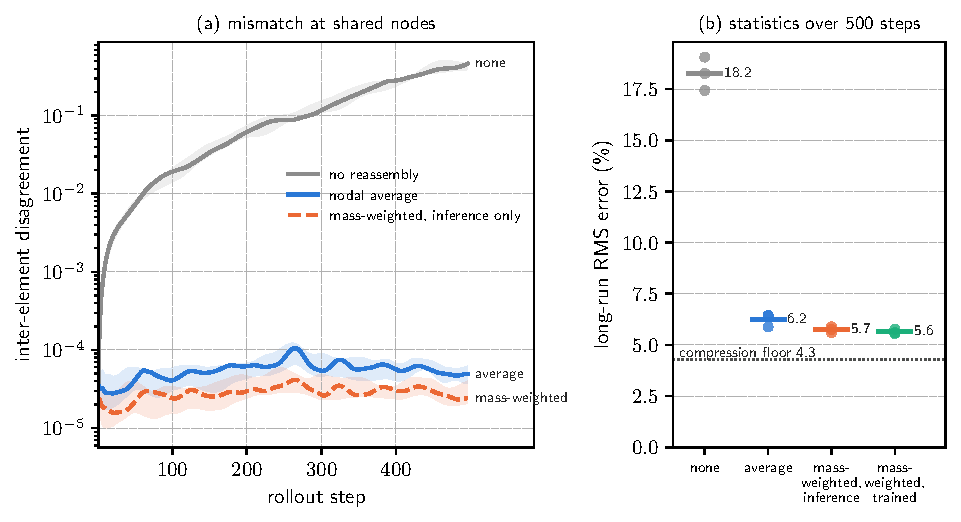
\includegraphics[width=\textwidth]{reassembly_study.pdf}
  \caption{Assembly of element predictions, $\Rey=15{,}000$, three seeds per setting. (a) Disagreement between elements at shared nodes during the 496-step rollout, as a fraction of the predicted frame's field energy (mean and seed range). (b) RMS velocity error over the rollout for each seed (dots) and the mean (bars); the dotted line is the compression floor.}
  \label{fig:reassembly}
\end{figure}

\begin{figure}[!tbp]
  \centering
  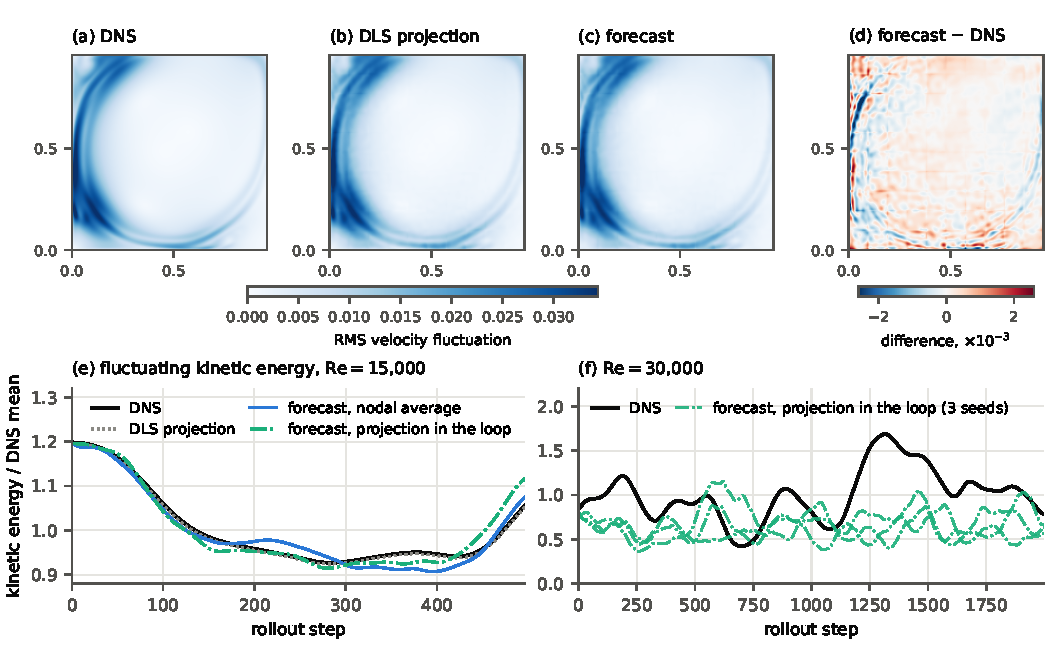
\includegraphics[width=\textwidth]{ldc_statistics.pdf}
  \caption{Long-run statistics on the lid-driven cavity. (a--d) RMS velocity fluctuation over the 496-step held-out rollout at $\Rey=15{,}000$ (seed 1): DNS, its DLS projection, the forecast trained through the mass-weighted projection, and the forecast minus the DNS. (e, f) Fluctuating kinetic energy over the rollout, relative to the DNS mean, at $\Rey=15{,}000$ (seed 1) and at $\Rey=30{,}000$ (10,000-snapshot record, three seeds).}
  \label{fig:ldc_stats}
\end{figure}

\subsection{Higher Reynolds number}
\label{sec:res_30k}
At $\Rey=30{,}000$ the same recipe does not generalize to the evaluation block (Table~\ref{tab:re30k}). With the first 4,500 snapshots, the model trained through the projection only matches persistence ($S=0.02$), and with nodal averaging it is worse than persistence ($S=-0.29$). The failure is one of generalization, not of optimization. The test loss at the end of training is 30 to 70 times the training loss, against 0.6--0.9 times at $\Rey=15{,}000$, and the record is far less stationary: the coefficient of variation of the training-block TKE is 0.35, against 0.09. Increasing the record to 10,000 snapshots raises the skill to $0.33\pm0.02$ over three seeds and lowers the 30-step error from 0.54 to $0.39\pm0.01$. The one-step error is still 1.6 times that of persistence, so the skill comes from errors that grow more slowly than the flow decorrelates, not from an accurate one-step map. Over the long rollout the two assemblies fail in opposite directions. Nodal averaging lets the energy grow to nine times the truth, whereas the projection-trained model dissipates to $0.65\pm0.06$ of it (Fig.~\ref{fig:ldc_stats}f). Decoupled weight decay \cite{loshchilov2019adamw} of $10^{-2}$, and Gaussian noise of standard deviation 0.01 on the fed-back state, both gave slightly worse forecasts (skill 0.28 and 0.26). The amount of training data is the only change so far that has improved the forecast. The frequency extrapolation of Ref.~\cite{morton2026scitech} again has no forecast skill ($S=-3.4$), but because it replays the true dynamics of the training record, its long-run RMS error, 23.4\%, is lower than the transformer's. At this Reynolds number the model forecasts better than the extrapolation but does not yet match its long-run statistics. The two records are evaluated on different blocks, but persistence scores almost the same on both (0.379 and 0.381).

\begin{table}[!tbp]
  \centering
  \small
  \caption{$\Rey=30{,}000$, p99m10, held-out split. Persistence: $\varepsilon_1=0.026$. Energy ratio is the mean predicted-to-true fluctuating energy over the free rollout.}
  \label{tab:re30k}
  \begin{tabular}{lcl ccccc}
    \toprule
    Snapshots & Floor, \% & Assembly & $S$ & $\varepsilon_{1}$ & $\varepsilon_{30}$ & RMS error, \% & Energy ratio \\
    \midrule
    4,500 & 6.80 & projection in the loop & 0.02 & 0.072 & 0.54 & 31.4 & 0.70 \\
    10,000 & 6.25 & nodal average & 0.11 & 0.027 & 0.58 & 252 & 9.18 \\
    10,000 & 6.25 & projection in the loop\textsuperscript{a} & 0.33(2) & 0.041(2) & 0.39(1) & 29.0(26) & 0.65(6) \\
    10,000 & 6.25 & frequency extrapolation \cite{morton2026scitech} & $-3.41$ & 1.68 & 1.67 & 23.4 & 1.13 \\
    \bottomrule
  \end{tabular}

  \smallskip
  {\footnotesize \textsuperscript{a}Mean over three seeds, with the standard deviation in the last digits in parentheses; the other rows are seed 1.}
\end{table}

\subsection{Challenge 2.1 cavity PIV}
\label{sec:res_challenge}
The test outputs of the challenge are withheld. We therefore score forecasts on 30 sequences cut from the held-out end of the training record (snapshots 11,520--12,799). The sequences start every 40 snapshots, so their forecast windows do not overlap. Each sequence gives 70 frames and asks for the next 30, as in the challenge; our model uses the last $\tau$ of the 70. All methods are scored with the official NMSE on the full $154\times51$ grid. A model whose mesh does not cover the grid forecasts the mean flow in the strip it cannot represent, which is what its submission would have to contain. The DMD baseline follows the official procedure; our implementation reproduces the official MATLAB routine to $10^{-14}$ on the challenge's test inputs. Table~\ref{tab:challenge} and Fig.~\ref{fig:challenge} summarize the results.

This flow is far less predictable than the lid-driven cavity. The field changes by nearly its own magnitude from one frame to the next, partly through measurement noise. Persistence already scores an NMSE of 0.60 at the first step, exceeds 1 from the third, and settles near 2 once the flow has decorrelated. The useful reference beyond a few steps is therefore the mean flow, whose NMSE is 1 at every step. DMD beats it only for the first five steps, and its 30-step mean NMSE is 1.09. The challenge paper reports that its LSTM baseline also exceeds an NMSE of 1 by lead 13 on the official test sequences \cite{schmidt2026challenge}.

The element-token transformer with the mass-weighted projection in the loop stays below the mean-flow forecast at every lead time, in each of three seeds. Its 30-step mean NMSE is $0.765\pm0.023$, against 1.09 for DMD, 0.96 for an earlier element-local temporal transformer, and 1.02 for a global temporal transformer. Its first-step NMSE is 0.34, against 0.48 for DMD. The improvement is not an artifact of damping toward the mean, which NMSE rewards once predictability is lost: the pattern correlation between forecast and truth at step 10 is 0.52, against 0.28 for DMD. The forecast does lose amplitude as it loses predictability, which Sec.~\ref{sec:tradeoff} examines.

Single-seed ablations, on the zero-weight variant of the basis, showed what matters. Reducing the model from 7.4 million parameters to 1.9 million, or to 0.25 million, left the 30-step mean unchanged (0.77, 0.78, and 0.77), and training on all 10,348 windows instead of 3,000 lowered it from 0.83 to 0.77. A longer input history hurt: with 8 or 16 input frames the held-out loss reached its minimum after 5 and 3 epochs, and the 30-step mean rose to 0.80 and 0.86. The seed-to-seed range of the reference recipe, 0.742--0.789, sets the resolution of these comparisons.

\begin{table}[!tbp]
  \centering
  \small
  \caption{Challenge 2.1 on 30 held-out sequences: official NMSE on the full $154\times51$ grid, mean over sequences. The element-token model has 1.9 million parameters and $\tau=4$, and is trained on all 10,348 windows.}
  \label{tab:challenge}
  \begin{tabular}{lccccc}
    \toprule
    Method & Step 1 & Step 5 & Step 10 & Step 30 & Mean 1--30 \\
    \midrule
    Persistence & 0.60 & 1.80 & 2.11 & 1.95 & 1.90 \\
    Mean flow & 1.00 & 1.00 & 1.00 & 1.00 & 1.00 \\
    DMD, 25 modes (baseline) & 0.48 & 0.99 & 1.18 & 1.13 & 1.09 \\
    DLS projection of truth (floor) & 0.037 & 0.036 & 0.038 & 0.037 & 0.036 \\
    \midrule
    Element-local temporal transformer\textsuperscript{a} & 0.38 & 0.97 & 1.02 & 1.00 & 0.96 \\
    Global temporal transformer\textsuperscript{a} & 0.56 & 0.90 & 0.99 & 1.27 & 1.02 \\
    Element-token transformer, projection in the loop\textsuperscript{b} & 0.34 & 0.58 & 0.76 & 0.90 & 0.77 \\
    \bottomrule
  \end{tabular}

  \smallskip
  {\footnotesize \textsuperscript{a}Single seed, original mesh ($151\times49$ of the $154\times51$ points); mean flow in the uncovered strip. \textsuperscript{b}Mean of three seeds, whose 30-step means are 0.742, 0.789, and 0.763.}
\end{table}

\begin{figure}[!tbp]
  \centering
  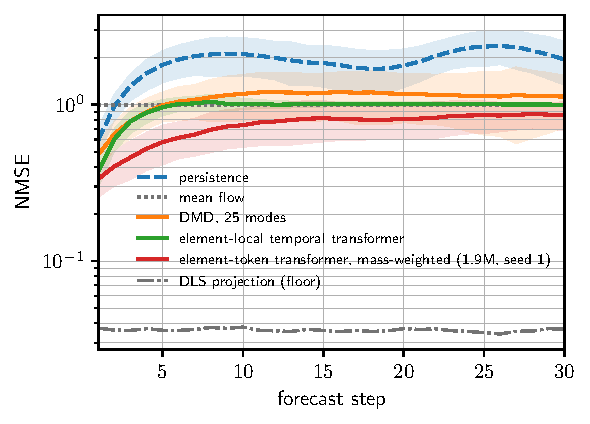
\includegraphics[width=0.6\textwidth]{challenge_heldout.pdf}
  \caption{Challenge 2.1 forecast error on 30 held-out sequences: official NMSE on the full grid; lines are means over sequences and bands are $\pm$ one standard deviation. The element-token transformer (1.9 million parameters, mass-weighted projection in the loop, seed 1) stays below the mean-flow forecast at every lead time.}
  \label{fig:challenge}
\end{figure}

\subsection{Forecast error and fluctuation recovery}
\label{sec:tradeoff}
The Challenge 2.1 forecasts lose amplitude as they lose skill, and NMSE rewards this. The reason is exact. For one sequence at lead $k$, let $E_k=\|\hat{\mathbf{q}}_k\|^2/\|\mathbf{q}_k\|^2$ be the energy ratio of the mean-removed forecast and $c_k=\langle\hat{\mathbf{q}}_k,\mathbf{q}_k\rangle/(\|\hat{\mathbf{q}}_k\|\,\|\mathbf{q}_k\|)$ its pattern correlation with the truth. Then
\begin{equation}
  \mathrm{NMSE}_k=1+E_k-2c_k\sqrt{E_k}=1-c_k^2+\bigl(c_k-\sqrt{E_k}\bigr)^2 .
  \label{eq:nmse_id}
\end{equation}
This is Murphy's decomposition of the mean-square-error skill score \cite{murphy1988skill}, and the law of cosines behind the Taylor diagram \cite{taylor2001diagram}. For a given correlation, the NMSE is smallest when the forecast carries the energy $E_k=c_k^2$, and the minimum is $1-c_k^2$. A forecast with the true energy scores $2(1-c_k)$. This exceeds the mean-flow value of 1 whenever $c_k<1/2$, however realistic the forecast's statistics.

The deterministic models are close to this optimum. Over the three seeds, the correlation falls from 0.81 at the first step to 0.52 at step 10 and 0.32 at step 30. Over the same steps the energy ratio falls from 0.68 to 0.35 and 0.18, tracking $c_k^2$ (0.66, 0.27, 0.10). Averaged over sequences and steps, the correlation term $1-c_k^2$ accounts for 0.718 of the mean NMSE of 0.765, and the amplitude term for the remaining 0.047. A model trained on a mean-square loss approximates the conditional mean of the future state, and Eq.~\eqref{eq:nmse_id} shows what this implies for amplitude. Its loss of energy is the NMSE-optimal response to its own correlation, not a failure of training. The NMSE can then be lowered appreciably only by raising the correlation, and energy can be recovered at fixed correlation only by raising the NMSE.

Table~\ref{tab:tradeoff} and Fig.~\ref{fig:cavity_stats} show what this means for long free rollouts. The DLS projection of the truth is within the sampling floor in every statistic except the spatial spectrum, where the finite enrichment removes the smallest scales. The forecasts are far from it. Within about 30 steps the fluctuating energy falls to a fifth of the truth and stays there ($0.21\pm0.02$ over the seeds). The rollout settles onto a nearly periodic state: almost all of its spectral power lies in a single tone and its harmonics, at 0.95 and 0.96~kHz for two seeds and at 1.52~kHz for the third. These are the second and third Rossiter tones of the cavity, which Zhang et al.~\cite{zhang2020samm} identify as its most energetic. The measured spectrum peaks at 0.94 and 1.54~kHz, and the modified Rossiter equation \cite{heller1971cavity} with the constants of Ref.~\cite{zhang2020samm} gives 0.96 and 1.55~kHz for a free-stream velocity of 200~m/s. The model has therefore learned the resonance of the cavity, but the broadband content that carries most of the measured energy is gone (Fig.~\ref{fig:cavity_stats}e). The RMS map keeps the outline of the shear layer at reduced amplitude, with an error of 8 times its sampling floor, and the spectral shapes are 55 and 54 times their floors. About a third of the spatial-spectrum distance comes from scales that no forecast can predict (Sec.~\ref{sec:eval}): restricted to wavelengths above five grid points, it is 35--39 times the floor. The gap between the forecasts and their basis is therefore set by the training objective, not by the representation.

An energy constraint restores the amplitude but not the dynamics. We add to the loss a term that penalizes the error in each frame's field energy, $\beta\,(\|\hat{\mathbf{u}}\|-\|\mathbf{u}\|)^2$, computed with $\lambda=0$ in Eq.~\eqref{eq:loss}. For a forecast whose only freedom is its amplitude, the combined loss is smallest at $\sqrt{E}=(c+\beta)/(1+\beta)$, which interpolates between the NMSE optimum ($\beta=0$) and the true energy ($\beta\rightarrow\infty$). With $\beta=1$ (one seed), the 30-step forecasts carry 0.64 of the true energy, close to the 0.56 predicted from their correlation, which is unchanged at 0.47. The NMSE rises from 0.765 to 0.879, as Eq.~\eqref{eq:nmse_id} requires. Over the free rollout the energy ratio rises to 0.71 and the RMS-map error falls from 8 to 4 times its floor, but the spectral shapes remain 58 and 40 times their floors. The term moves the model along Eq.~\eqref{eq:nmse_id}, as a gain applied to the forecast would, without adding information. It restores how much a deterministic forecast fluctuates, but changes little about how.

\begin{table}[!tbp]
  \centering
  \small
  \setlength{\tabcolsep}{3pt}
  \caption{Forecast error and fluctuation recovery on Challenge 2.1, 1.9 M model. Left: 30-step forecasts of the 30 held-out sequences, with mean NMSE over steps 1--30, energy ratio $E$, and pattern correlation $c$. Right: free rollout over the held-out block (Sec.~\ref{sec:eval}), with the fluctuating-energy ratio and the other distances as multiples of their sampling floors (RMS map 0.072; spatial and frequency spectrum shape 0.30 and 0.37~dB; distribution shape 0.054).}
  \label{tab:tradeoff}
  \begin{tabular}{lcccccccc}
    \toprule
    & \multicolumn{3}{c}{30-step forecasts} & \multicolumn{5}{c}{Free rollout} \\
    \cmidrule(lr){2-4}\cmidrule(lr){5-9}
    Configuration & NMSE & $E$ & $c$ & Energy & RMS map & $x$ spectrum & $t$ spectrum & PDF \\
    \midrule
    True flow, other segments & -- & -- & -- & 0.96 & 1 & 1 & 1 & 1 \\
    DLS projection of truth & -- & -- & -- & 0.97 & 0.3 & 17.8 & 0.7 & 0.3 \\
    Reference, three seeds & $0.765\pm0.023$ & $0.30\pm0.03$ & 0.47 & $0.21\pm0.02$ & 8.1 & 55 & 54 & 4.8 \\
    \quad + energy term, $\beta=1$, one seed & 0.879 & 0.64 & 0.47 & 0.71 & 4.0 & 58 & 40 & 4.3 \\
    \bottomrule
  \end{tabular}
\end{table}

\begin{figure}[!tbp]
  \centering
  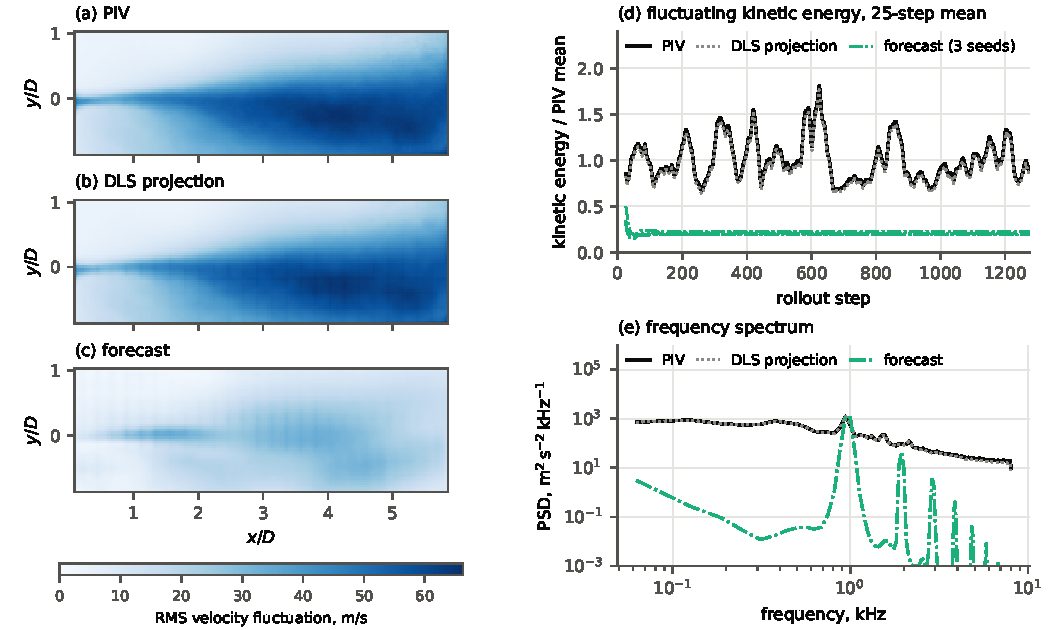
\includegraphics[width=\textwidth]{cavity_statistics.pdf}
  \caption{Long-run statistics of free rollouts on Challenge 2.1 over the held-out block (1,276 steps). (a--c) RMS velocity fluctuation of the PIV data, of its DLS projection, and of the forecast (seed 1). (d) Fluctuating kinetic energy relative to the PIV mean, as a 25-step moving average, for three seeds. (e) Frequency spectrum averaged over the grid (seed 1).}
  \label{fig:cavity_stats}
\end{figure}

%=====================================================================================
\section{Discussion}
\label{sec:discussion}
The results support treating the data-enriched finite element basis as more than a compressor. The element structure supplies the tokens, so the forecast is posed on local, position-aware units that share one set of weights. The mass matrix supplies the metric. For training it needs a ridge to keep rollouts stable, and on an ill-conditioned basis that ridge carries most of the loss, so its value trades short-horizon error against long-run statistics. The assembly supplies consistency. Combining element predictions by the field-metric projection improved every short-horizon metric in every seed, and training through that projection improved the 30-step error and its consistency across seeds. None of these components uses the governing equations.

The same recipe transferred to experimental data without changes to the architecture. On the Challenge 2.1 cavity its error stays below that of the mean-flow forecast throughout the 30-step window, and its pattern correlation with the truth is well above DMD's. Narrower networks forecast as well as the full one, and a longer input history made the model overfit within a few epochs. The record contains less information that generalizes than the full network can absorb.

Two limitations stand out. First, at $\Rey=30{,}000$ the limiting factor is the amount and stationarity of the training record rather than the architecture: more data was the only change that improved the forecast. Second, a deterministic model trained on a mean-square loss converges toward the conditional mean of the future state. Where predictability is short, as in the Challenge 2.1 cavity and at $\Rey=30{,}000$, its forecasts lose amplitude as they lose skill, and its long rollouts keep 21\% and 65\% of the true fluctuating energy. Section~\ref{sec:tradeoff} shows that this loss of energy is the NMSE-optimal response to the forecast's own correlation, and that an energy penalty restores the amplitude without restoring the spectrum. NMSE therefore rewards what turbulence statistics penalize. Generative or stochastic forecasting on the same element tokens \cite{kohl2023acdm,lippe2023pderefiner} is the natural way to keep both.

%=====================================================================================
\section{Conclusions}
\label{sec:conclusions}
We posed transformer forecasting of turbulent flow on the elements of a data-enriched finite element basis, with one token per element and attention over space. On the lid-driven cavity at $\Rey=15{,}000$, with 2,662 latent coefficients (four times fewer than our prior work), the model forecasts 30 steps ahead with a mean relative field error of 3.8\%, against 32.4\% for persistence. The error is consistent across forecasts and across seeds, and the 500-step RMS velocity field is within 1.4 percentage points of the compression floor. Two finite element ingredients were responsible for much of the improvement over the original formulation: a field-energy metric from the basis's mass matrix, and a mass-weighted projection of the element predictions, applied inside the training rollout. Attention over element tokens outperformed a global temporal transformer on the same latent space. At $\Rey=30{,}000$ the recipe overfits a short training record; a longer record raises the 30-step skill to 0.33, but the long rollout still loses a third of its energy. On the Challenge 2.1 cavity PIV, a 1.9-million-parameter version of the model has a mean 30-step NMSE of 0.77 on held-out sequences, against 1.09 for the DMD baseline and 1.0 for the mean flow. The remaining gap is amplitude and spectral content: the forecasts damp toward the mean as predictability is lost, and long rollouts collapse onto a single Rossiter tone.

\section*{Acknowledgments}
This project is supported by the Office of Naval Research under grant number N00014-23-1-2398, with Leighton Meyers as Program Officer; and the SMART scholarship to Caleb Morton, funded by the Naval Air Warfare Center Aircraft Division at Patuxent River Naval Air Station. The authors acknowledge the use of DoD HPCMP computing resources. The authors also thank Dr. Sachin Kumar for helpful discussions and insights on this work.

\bibliography{references}

\end{document}
